\newif\ifshowsolutions
\showsolutionstrue
\documentclass{article}
\usepackage{listings}
\usepackage{amsmath}
\usepackage{subfig}
\usepackage{amsthm}
\usepackage{amsmath}
\usepackage{amssymb}
\usepackage{graphicx}
\usepackage{mdwlist}
\usepackage{geometry}
\usepackage{titlesec}
\usepackage{palatino}
\usepackage{mathrsfs}
\usepackage{fancyhdr}
\usepackage{paralist}
\usepackage{todonotes}
\usepackage{tikz}
\usepackage{float} % Place figures where you ACTUALLY want it
\usepackage{comment} % A hack to toggle sections
\usepackage{ifthen}
\usepackage{mdframed}
\usepackage{verbatim}
\usepackage{listings}
\usepackage{bbm}
\usepackage{upquote} % Prevents backticks replacing single-quotes in verbatim
\usepackage[strings]{underscore}
\usepackage[english]{babel}
\usepackage[colorlinks=true]{hyperref}
\usetikzlibrary{positioning,shapes,backgrounds}

\geometry{margin=1in}
\geometry{headheight=2in}
\geometry{top=2in}

\setlength{\marginparwidth}{2.15cm}
\setlength{\parindent}{0em}
\setlength{\parskip}{0.6\baselineskip}

\rhead{}
\lhead{}

% Spacing settings.
\titlespacing\section{0pt}{12pt plus 2pt minus 2pt}{0pt plus 2pt minus 2pt}
\titlespacing\subsection{0pt}{12pt plus 4pt minus 2pt}{0pt plus 2pt minus 2pt}
\titlespacing\subsubsection{0pt}{12pt plus 4pt minus 2pt}{0pt plus 2pt minus 2pt}
\renewcommand{\baselinestretch}{1.15}

% Shortcuts for commonly used operators.
\newcommand{\E}{\mathbb{E}}
\newcommand{\Var}{\operatorname{Var}}
\newcommand{\Cov}{\operatorname{Cov}}
\newcommand{\Bias}{\operatorname{Bias}}
\DeclareMathOperator{\argmin}{arg\,min}
\DeclareMathOperator{\argmax}{arg\,max}

% Do not number subsections and below.
\setcounter{secnumdepth}{1}

% Custom format subsection.
\titleformat*{\subsection}{\large\bfseries}

% Set up the problem environment.
\newcounter{problem}[section]
\newenvironment{problem}[1][]
  {\begingroup
    \setlength{\parskip}{0em}
    \refstepcounter{problem}\par\addvspace{1em}\textbf{Problem~\Alph{problem}\!
    \ifthenelse{\equal{#1}{}}{}{ [#1 points]}:}
  \endgroup}

% Set up the subproblem environment.
\newcounter{subproblem}[problem]
\newenvironment{subproblem}[1][]
  {\begingroup
    \setlength{\parskip}{0em}
    \refstepcounter{subproblem}\par\medskip\textbf{\roman{subproblem}.\!
    \ifthenelse{\equal{#1}{}}{}{ [#1 points]:}}
  \endgroup}

% Set up the teachers and materials commands.
\newcommand\teachers[1]
  {\begingroup
    \setlength{\parskip}{0em}
    \vspace{0.3em} \textit{\hspace*{2em} TAs responsible: #1} \par
  \endgroup}
\newcommand\materials[1]
  {\begingroup
    \setlength{\parskip}{0em}
    \textit{\hspace*{2em} Relevant materials: #1} \par \vspace{1em}
  \endgroup}

% Set up the hint environment.
\newenvironment{hint}[1][]
  {\begin{em}\textbf{Hint: }}
  {\end{em}}


% Set up the solution environment.
\ifshowsolutions
  \newenvironment{solution}[1][]
    {\par\medskip \begin{mdframed}\textbf{Solution~\Alph{problem}#1:} \begin{em}}
    {\end{em}\medskip\end{mdframed}\medskip}
  \newenvironment{subsolution}[1][]
    {\par\medskip \begin{mdframed}\textbf{Solution~\Alph{problem}#1.\roman{subproblem}:} \begin{em}}
    {\end{em}\medskip\end{mdframed}\medskip}
\else
  \excludecomment{solution}
  \excludecomment{subsolution}
\fi



%%%%%%%%%%%%%%%%%%%%%%%%%%%%%%
% HEADER
%%%%%%%%%%%%%%%%%%%%%%%%%%%%%%

\chead{
  {\vbox{
      \vspace{2mm}
      \large
      Machine Learning \& Data Mining \hfill
      Caltech CS/CNS/EE 155 \hfill \\[1pt]
      Set 3\hfill
      January $28^\text{th}$, 2023 \\
    }
  }
}

\begin{document}
\pagestyle{fancy}



%%%%%%%%%%%%%%%%%%%%%%%%%%%%%%
% POLICIES
%%%%%%%%%%%%%%%%%%%%%%%%%%%%%%

\section*{Policies}
\begin{itemize}
	\item Due 9 PM PST, January $28^\text{th}$ on Gradescope. 
	\item You are free to collaborate on all of the problems, subject to the collaboration policy stated in the syllabus.
	\item In this course, we will be using Google Colab for code submissions. You will need a Google account.
\end{itemize}

\section*{Submission Instructions}
\begin{itemize}
	\item Submit your report as a single .pdf file to Gradescope, under "Set 3 Report". 
	\item In the report, \textbf{include any images generated by your code} along with your answers to the questions.
	\item Submit your code by \textbf{sharing a link in your report} to your Google Colab notebook for each problem (see naming instructions below). Make sure to set sharing permissions to at least "Anyone with the link can view". \textbf{Links that can not be run by TAs will not be counted as turned in.} Check your links in an incognito window before submitting to be sure. 
	\item For instructions specifically pertaining to the Gradescope submission process, see \url{https://www.gradescope.com/get_started#student-submission}.
\end{itemize}

\section*{Google Colab Instructions}
For each notebook, you need to save a copy to your drive.
\begin{enumerate}
	\item Open the github preview of the notebook, and click the icon to open the colab preview.
	\item On the colab preview, go to File $\rightarrow$ Save a copy in Drive.
	\item Edit your file name to “lastname_firstname_set_problem”, e.g.”yue_yisong_set3_prob2.ipynb”
\end{enumerate}

%%%%%%%%%%%%%%%%%%%%%%%%%%%%%%
% PROBLEM 1
%%%%%%%%%%%%%%%%%%%%%%%%%%%%%%

\newpage
\section{Decision Trees [30 Points]}
\materials{Lecture 5}

\problem[7]
Consider the following data, where given information about some food you must predict whether it is healthy:

\begin{table}[ht]
\centering
\begin{tabular}{c | c c c | c}
\hline
No. & Package Type & Unit Price $>$ \$5 & Contains $>$ 5 grams of fat & Healthy? \\ [0.5ex]
\hline
1 & Canned & Yes & Yes & No  \\
2 & Bagged & Yes & No  & Yes \\
3 & Bagged & No  & Yes & Yes \\
4 & Canned & No  & No  & Yes \\ [1ex]
\hline
\end{tabular}
\end{table}

Train a decision tree by hand using top-down greedy induction. Use \emph{entropy} (with natural log) as the impurity measure.  Since the data can be classified
without error, the stopping criterion will be no impurity in the leaves.

Submit a drawing of your tree showing the impurity reduction yielded by each split (including root) in your decision tree.

\begin{solution}


\end{solution}

\problem[4]
Compared to a linear classifier, is a decision tree always preferred for classification problems? Briefly explain why or why not. If not, draw a simple 2-D dataset that can be perfectly classified by a simple linear classifier but which requires an overly complex decision tree to perfectly classify.

\begin{solution}
  
\end{solution}

\problem[15]
Consider the following 2D data set:
\begin{figure}[H]
    \begin{center}
    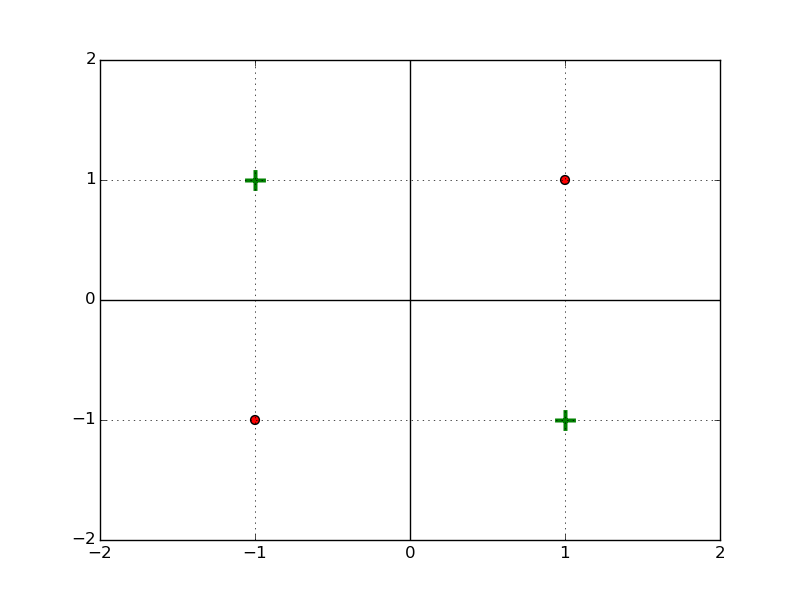
\includegraphics[width=3.3in]{plots/3C.png}
    \end{center}
    \end{figure}

\subproblem[5] Suppose we train a decision tree on this dataset using top-down greedy induction, with the Gini index as
the impurity measure. We define our stopping condition to be if no split of a node
results in any reduction in impurity. Submit a drawing of the resulting tree.  What is its classification error ((number of misclassified points) / (number of total points))?

\subproblem[5] Submit a drawing of a two-level decision tree that classifies the above dataset with zero classification error.  (You don't need to use any particular training algorithm to produce the tree.)

Is there any impurity measure (i.e. any function that maps the data points under a particular node in a tree to a real number) that would have led top-down greedy induction with the same stopping condition to produce the tree you drew?  If so, give an example of one, and briefly describe its pros and cons as an impurity measure for training decision trees in general (on arbitrary datasets). 

\subproblem[5] Suppose there are 100 data points in some 2-D dataset. What is the largest number of unique thresholds (i.e., internal nodes) you might need in order to achieve zero classification training error (on the training set)? Please
justify your answer.

\begin{solution}

\end{solution}

\problem[4] Suppose in top-down greedy induction we want to split a leaf node that contains N data points composed of
D continuous features. What is the worst-case
complexity (big-O in terms of N and D) of the number of possible splits we must consider in order to find the one that most reduces impurity? Please justify your answer.

Note: Recall that at each node-splitting step in training a DT, you must consider all possible splits that you can make. While there are an infinite number of possible decision boundaries since we are using continuous features, there are not an infinite number of boundaries that result in unique child sets (which is what we mean by ``split'').

\begin{solution}
   
\end{solution}


\newpage


\section{Overfitting Decision Trees [30 Points, EC 7 Points]}
\materials{Lecture 5}

In this problem, you will use the Diabetic Retinopathy Debrecen Data Set, which contains features extracted from images to determine whether or not the images contain signs of diabetic retinopathy. Additional information about this dataset can be found at the link below:

\url{https://archive.ics.uci.edu/ml/datasets/Diabetic+Retinopathy+Debrecen+Data+Set}

In the following question, your goal is to predict the diagnosis of diabetic retinopathy, which is the final column in the data matrix.  Use the first 900 rows as training data, and the last
251 rows as validation data. Please feel free to use additional packages such as Scikit-Learn. Include your code in your submission.


\indent\problem[10] \smallskip 
Choose one of the following from i or ii: 

\noindent i. Train a decision tree classifier using Gini as the impurity measure and minimal leaf node size as early stopping criterion. Try different minimal leaf node sizes from 1 to 25 in increments of 1. Then, on a single plot, plot both training and test classification error versus leaf node size. To do this, fill in the \texttt{classification_err} and \texttt{eval_tree_based_model_min_samples} functions in the code template for this problem.


ii. Train a decision tree classifier using Gini as the impurity measure and maximal tree depth as early stopping criterion. Try different tree depths from 2 to 20 in increments of 1. Then, on a single plot, plot both training and test classification error versus tree depth. To do this, fill in the \texttt{eval_tree_based_model_max_depth} function in the code template for this problem.

\begin{solution}
 
\end{solution}

\problem[6]
For either the minimal leaf node size or maximum depth parameters in the previous problem, which parameter value minimizes the test error? What effects does early stopping have on the performance of a decision tree model?
Please justify your answer based on the plot you derived.

\begin{solution}
   
\end{solution}

\indent\problem[4] Choose one of the following from i or ii: \smallskip 

\noindent i. Train a random forest classifier using Gini as the impurity measure, minimal leaf node size as early stopping criterion, and 1,000 trees in the forest. Try different node sizes from 1 to 25 in increments of 1. Then, on a single plot, plot both training and test classification error versus
leaf node size.

ii. Train a random forest classifier using Gini as the impurity measure, maximal tree depth as early stopping criterion, and 1,000 trees in the forest. Try different tree depths from 2 to 20 in increments of 1. Then, on a single plot, plot both training and test classification error versus tree depth.

\begin{solution}

\end{solution}

\problem[6]
For either the minimal leaf node size or maximum depth parameters tested, which parameter value minimizes the random forest test error? What effects does early stopping have on the performance of a random forest model?
Please justify your answer based on the plot you derived.

\begin{solution}

\end{solution}

\problem[4]
Do you observe any differences between the curves for the random forest and decision tree plots? If so, explain what could account for these differences.

\begin{solution}

\end{solution}

\textbf{Extra Credit [7 points total] :} \problem\textbf{[5 points, Extra Credit]} Complete the other option for \textbf{Problem A }and \textbf{Problem C}.

\begin{solution}
   
\end{solution}

\problem\textbf{[2 points, Extra Credit] }For the stopping criterion tested in \textbf{Problem F}, which parameter value minimizes the decision tree and random forest test error respectively? 

\begin{solution}
   
\end{solution}



\newpage
\section{The AdaBoost Algorithm [40 points]}
\materials{Lecture 6}

In this problem, you will show that the choice of the $\alpha_t$ parameter in
the AdaBoost algorithm corresponds to greedily minimizing an exponential upper
bound on the loss term at each iteration.

\problem[3]
Let $h_t: \mathbb{R}^m \rightarrow \{-1,1\}$ be the weak classifier obtained at step $t$, and let $\alpha_t$ be
its weight. Recall that the final classifier is $$H(x) = \text{sign}(f(x)) = \text{sign} \left(\sum\limits_{i=1}^T \alpha_{t}h_t(x) \right).$$

Suppose $\{(x_1, y_1), ..., (x_N, y_N)\} \subset \mathbb{R}^m \times \{-1,1\}$ is our training dataset.  Show that the training set error of the final classifier can be bounded from
above if an an exponential loss function is used:

$$E = \frac{1}{N} \sum\limits_{i=1}^N \exp(-y_{i}f(x_i)) \geq \frac{1}{N} \sum\limits_{i=1}^N \mathbbm{1}(H(x_i) \neq y_i),$$

where $\mathbbm{1}$ is the indicator function.

\begin{solution}

\end{solution}

\problem[3]
Find $D_{T + 1}(i)$ in terms of $Z_t$, $\alpha_t$, $x_i$, $y_i$, and the classifier $h_t$, where $T$ is the last timestep and $t \in \{1, \ldots, T\}$. Recall that $Z_t$ is the normalization factor for distribution $D_{t+1}$:
$$Z_t = \sum\limits_{i=1}^N D_t(i) \exp(-\alpha_{t}y_{i}h_{t}(x_{i})).$$

\begin{solution}

\end{solution}

\problem[2]
Show that $E = \sum_{i=1}^N  \frac{1}{N} e^{\sum_{t=1}^T -\alpha_t y_i h_t(x_i)}.$

\begin{solution}

\end{solution}

\problem[5]
Show that
$$E = \prod\limits_{t=1}^T Z_t.$$

\begin{hint}
	Recall that $\sum_{i = 1}^N D_t(i) = 1$ because $D$ is a distribution.
\end{hint}

\begin{solution}

\end{solution}

\problem[5]
Show that the normalizer $Z_t$ can be written as
\[Z_t = (1 - \epsilon_t) \exp(-\alpha_t) + \epsilon_{t} \exp(\alpha_t)\]
where $\epsilon_t$ is the training set error of weak classifier $h_t$ for the weighted dataset:
\[\epsilon_t = \sum\limits_{i=1}^N D_t(i)\mathbbm1(h_t(x_i) \neq y_i).\]

\begin{solution}
	
\end{solution}

\problem[2]
We derived all of this because it is hard to directly minimize the training set error, but we can greedily minimize the upper bound $E$ on this error. Show that choosing $\alpha_t$
greedily to minimize $Z_t$ at each iteration leads to the choices in
AdaBoost:
$$\alpha_{t}^* = \frac{1}{2} \ln \left(\frac{1 - \epsilon_t}{\epsilon_t} \right).$$

\begin{solution}
	
\end{solution}

\begin{problem}[14]
    Implement the \texttt{GradientBoosting.fit()} and \texttt{AdaBoost.fit()} methods in the notebook provided for you. Some important notes and guidelines follow:
    \begin{itemize}
        \item For both methods, make sure to work with the class attributes provided to you. Namely, after \texttt{GradientBoosting.fit()} is called, \texttt{self.clfs} should be appropriately filled with the \texttt{self.n_clfs} trained weak hypotheses. Similarly, after \texttt{AdaBoost.fit()} is called, \texttt{self.clfs} and \texttt{self.coefs} should be appropriately filled with the \texttt{self.n_clfs} trained weak hypotheses and their coefficients, respectively.
        \item \texttt{AdaBoost.fit()} should additionally return an $(N, T)$ shaped numpy array \texttt{D} such that \texttt{D[:, t]} contains $D_{t+1}$ for each $t \in \{0, \ldots, \texttt{self.n_clfs}\}$.
        \item For the \texttt{AdaBoost.fit()} method, \textbf{use the 0/1 loss} instead of the exponential loss.
	\item The only Sklearn classes that you may use in implementing your boosting fit functions are the DecisionTreeRegressor and DecisionTreeClassifier, not GradientBoostingRegressor.
    \end{itemize}
\end{problem}

\begin{problem}[2]
    Describe and explain the behaviour of the loss curves for gradient boosting and for AdaBoost. You should consider two kinds of behaviours: the smoothness of the curves and the final values that the curves approach.
\end{problem}

\begin{solution}
  
\end{solution}

\begin{problem}[2]
    Compare the final loss values of the two models. Which performed better on the classification dataset?
\end{problem}

\begin{solution}
  
\end{solution}

\begin{problem}[2]
    For AdaBoost, where are the dataset weights the largest, and where are they the smallest?
\end{problem}
\begin{hint}
    Watch how the dataset weights change across time in the animation.
\end{hint}
\begin{solution}
   
\end{solution}

\newpage
\section{Convex Functions [7 points, EC 3 Points]}

\emph{This problem further develops the ideas of convex functions, and provides intuition for why convex optimization is so important for
 Machine Learning.}

Given a convex set $\mathcal{X}$, a function $f:\mathcal{X}\to\mathbb{R}$ is \textbf{convex} if for all $\textbf{x},\textbf{y}\in \mathcal{X}$ and all $t\in[0,1]$ :
\[f(t\textbf{x} + (1-t)\textbf{y}) \leq tf(\textbf{x}) + (1-t)f(\textbf{y})\]

\begin{problem}[3]
Let $\mathcal{X}$ be a convex set. If $f$ is a convex function, show that any local minimum of $f$ in $\mathcal{X}$ is also a global minimum.
\end{problem}

\begin{solution}
   
\end{solution}

\begin{problem}[4]
\emph{Using part A}, explain why convex loss functions are desirable when training learning models.
\end{problem}

\begin{solution}
   
\end{solution}
\problem\textbf{[3 points, Extra Credit] }
The Kullback-Leibler (KL) divergence is a measure of statistical distance between two probability distributions $(p, q)$, also called the relative entropy. KL divergence can be used to generate optimal parameters for visualization models (which we will also see in set 4).
\[\mathrm{KL}[P\|Q] = \sum_{x\in\mathcal{X}} p(x) \cdot \log \frac{p(x)}{q(x)}\]
Show that the KL divergence is a convex loss function. \\

\begin{hint}
    Use the log sum inequality
\end{hint}

\begin{solution}
   
\end{solution}
\end{document}